\section{Hit rates}
\label{sec:hitrates}

Hit rates increase with lumi.

\begin{figure}
  \begin{center}
    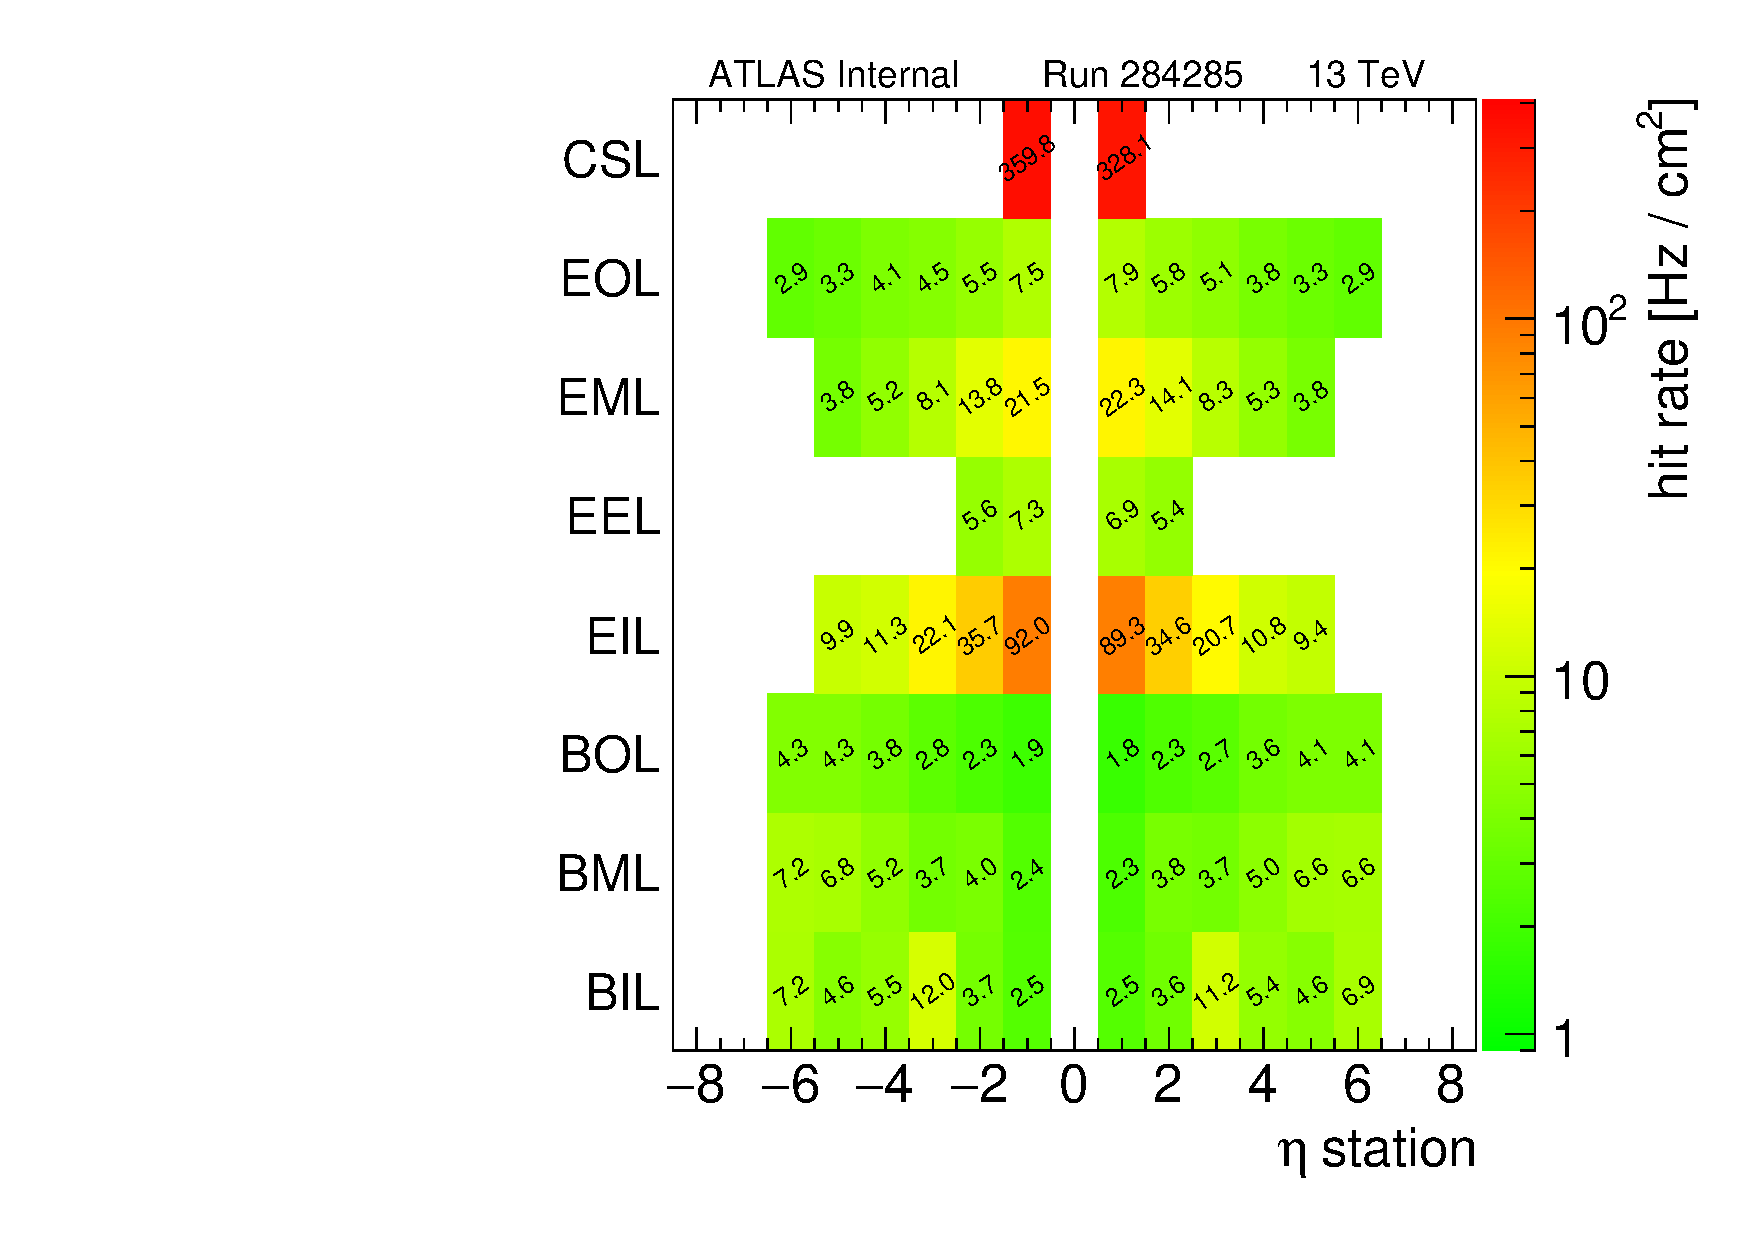
\includegraphics[width=0.45\textwidth]{./figures/rate_raw_vs_region_L_00284285.pdf}
    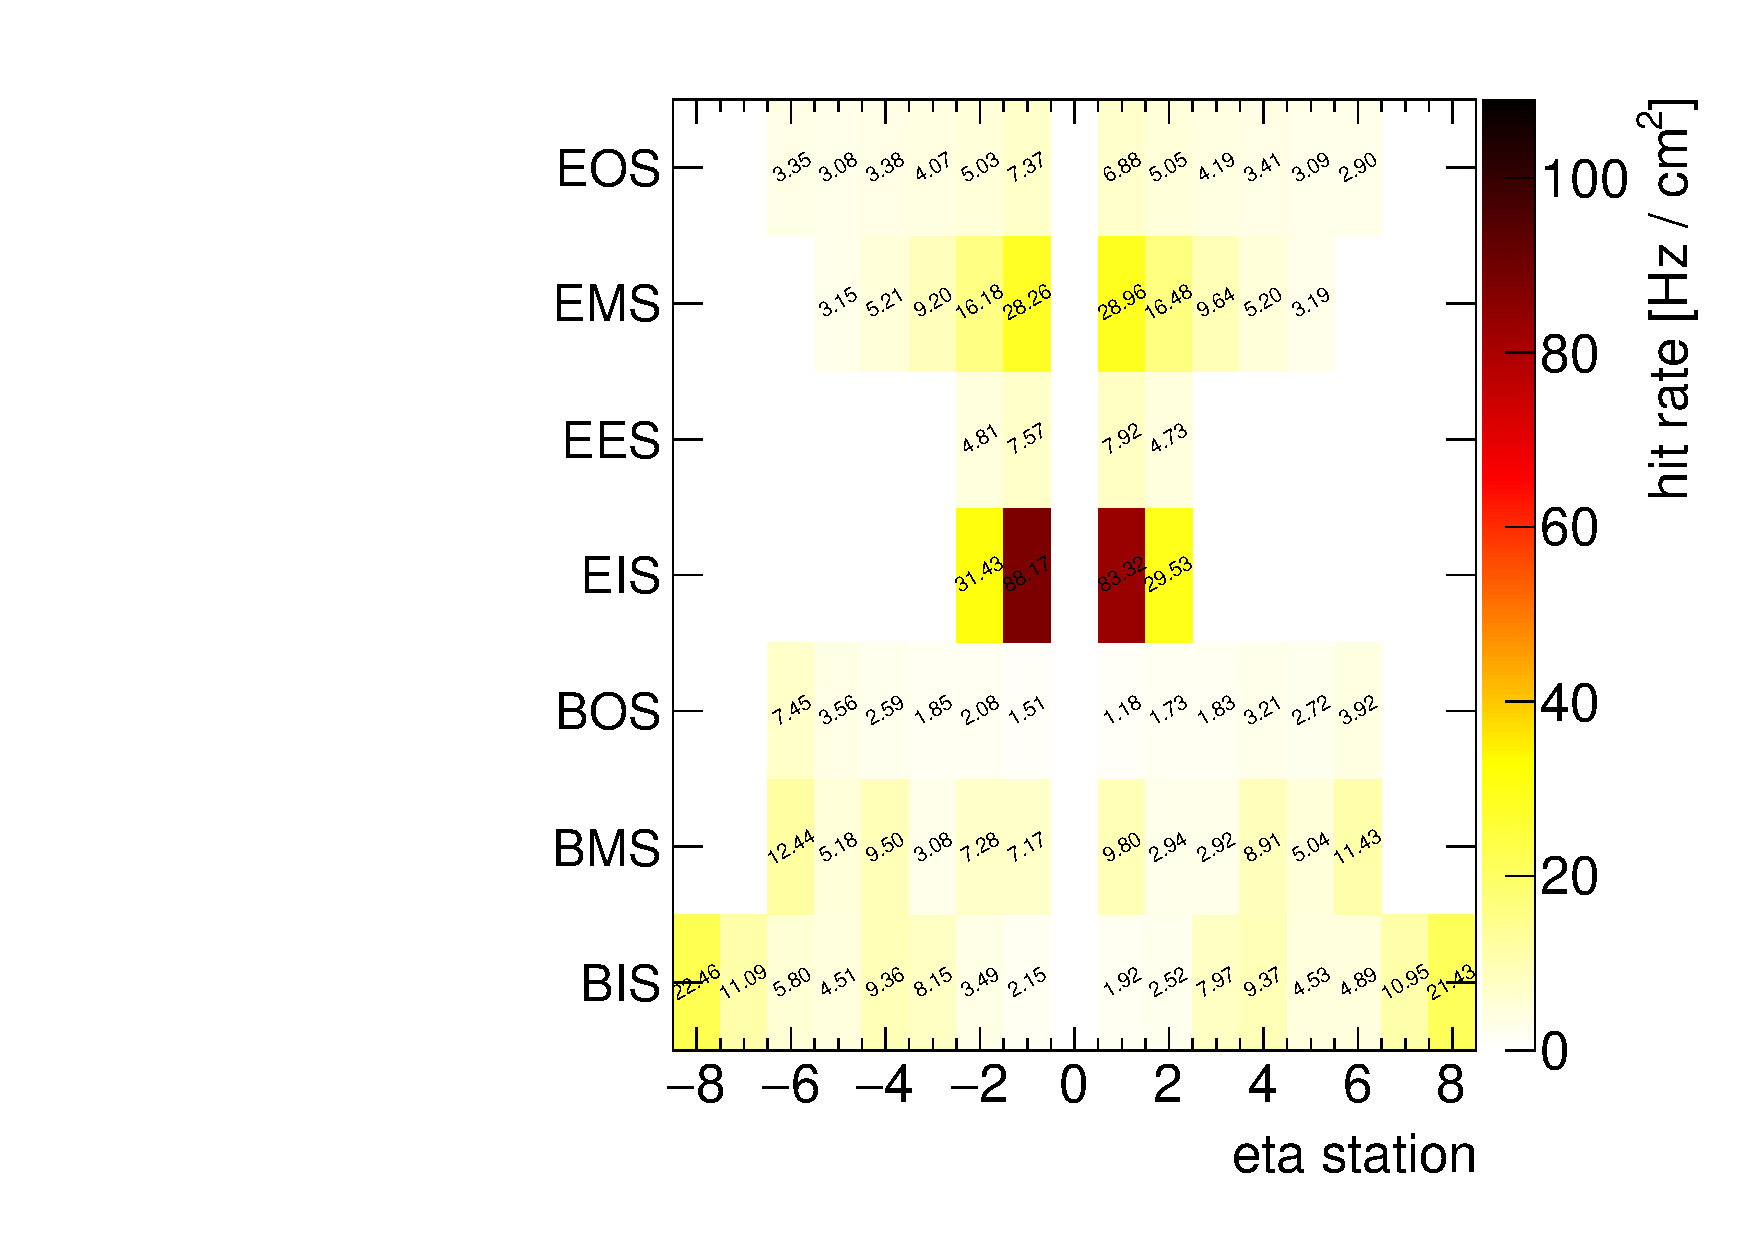
\includegraphics[width=0.45\textwidth]{./figures/rate_raw_vs_region_S_00284285.pdf}
    \caption{Total hit rate in the MDTs in Run 284285 in the largest regions of the detector. The rates are split into large sectors (left) and small sectors (right).}
    \label{fig:hitrates-vs-region-raw}
  \end{center}
\end{figure}

\begin{figure}
  \begin{center}
    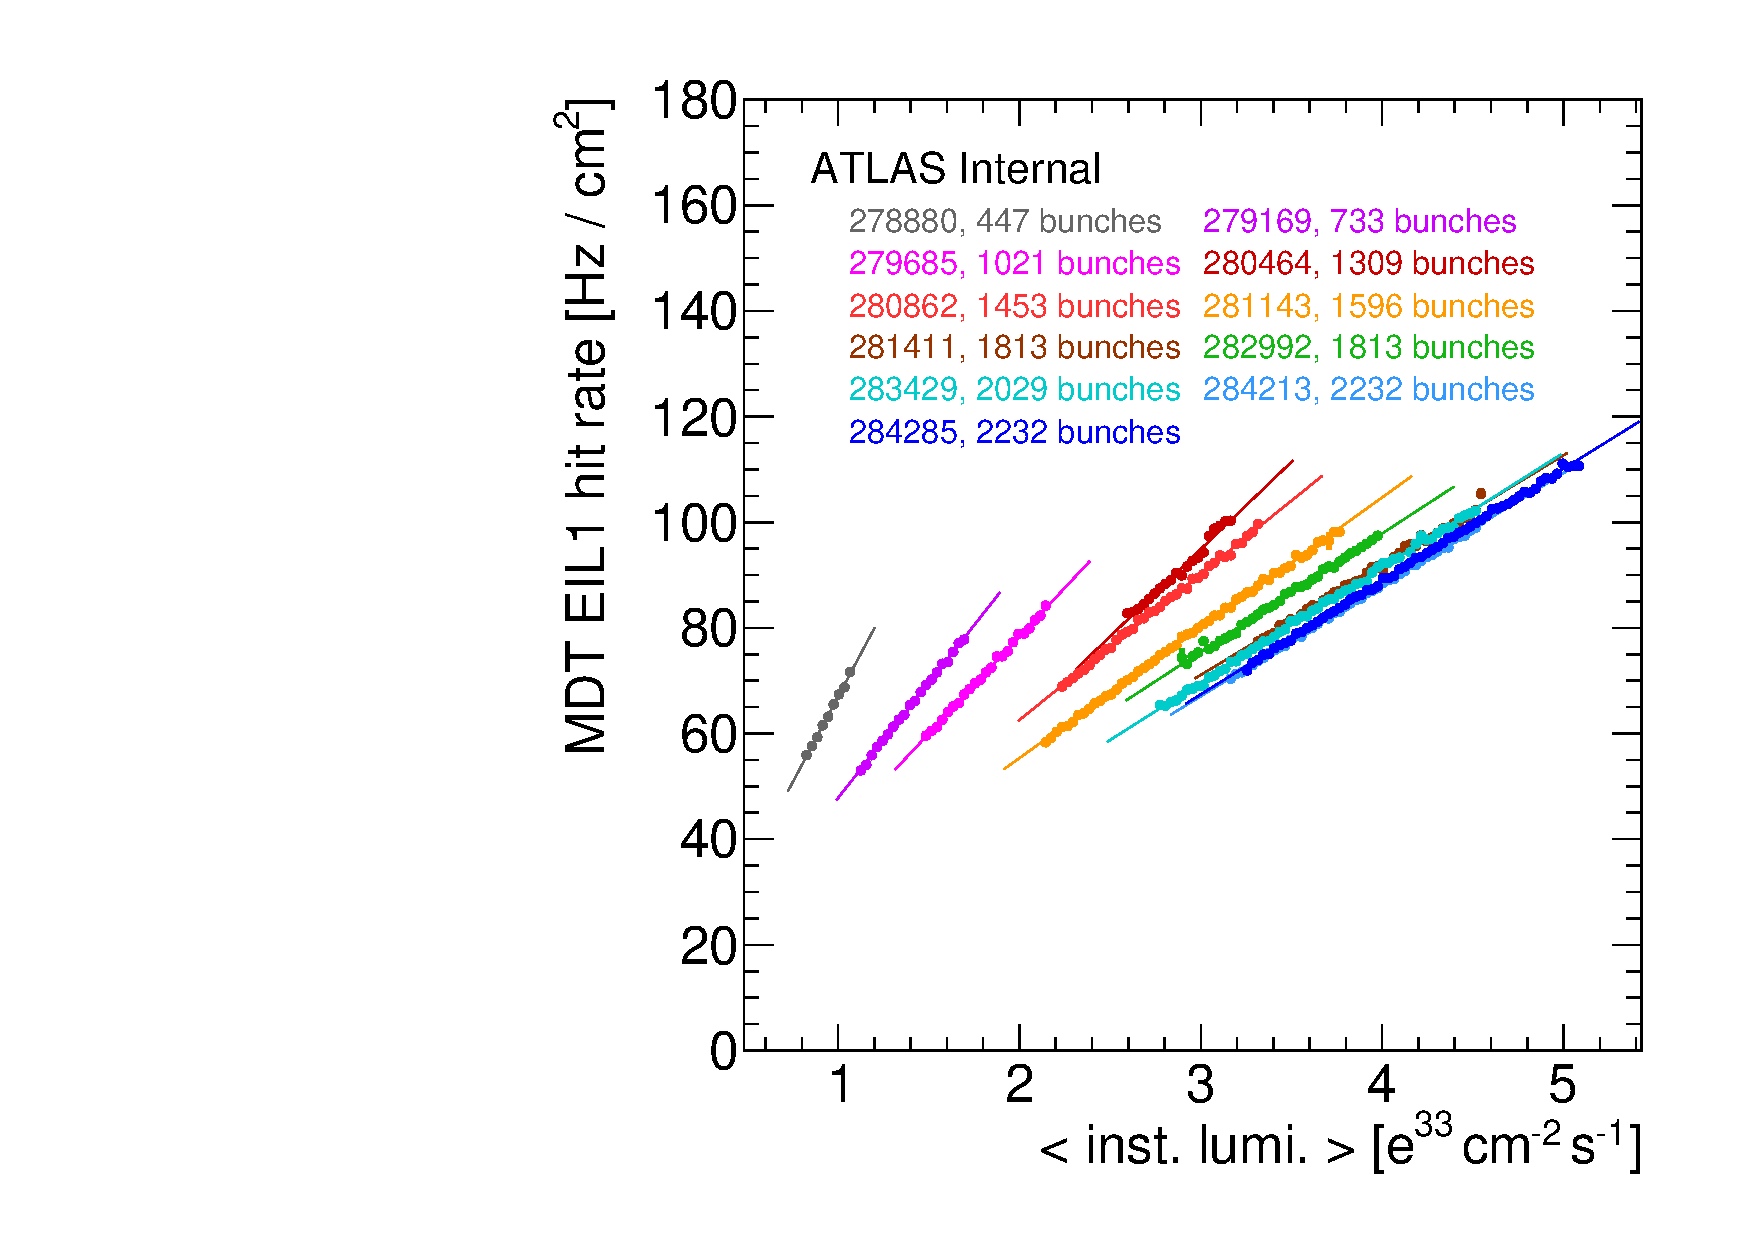
\includegraphics[width=0.45\textwidth]{./figures/rate_raw_vs_lumi_vs_evts_mdt_EIL1_overlay.pdf}
    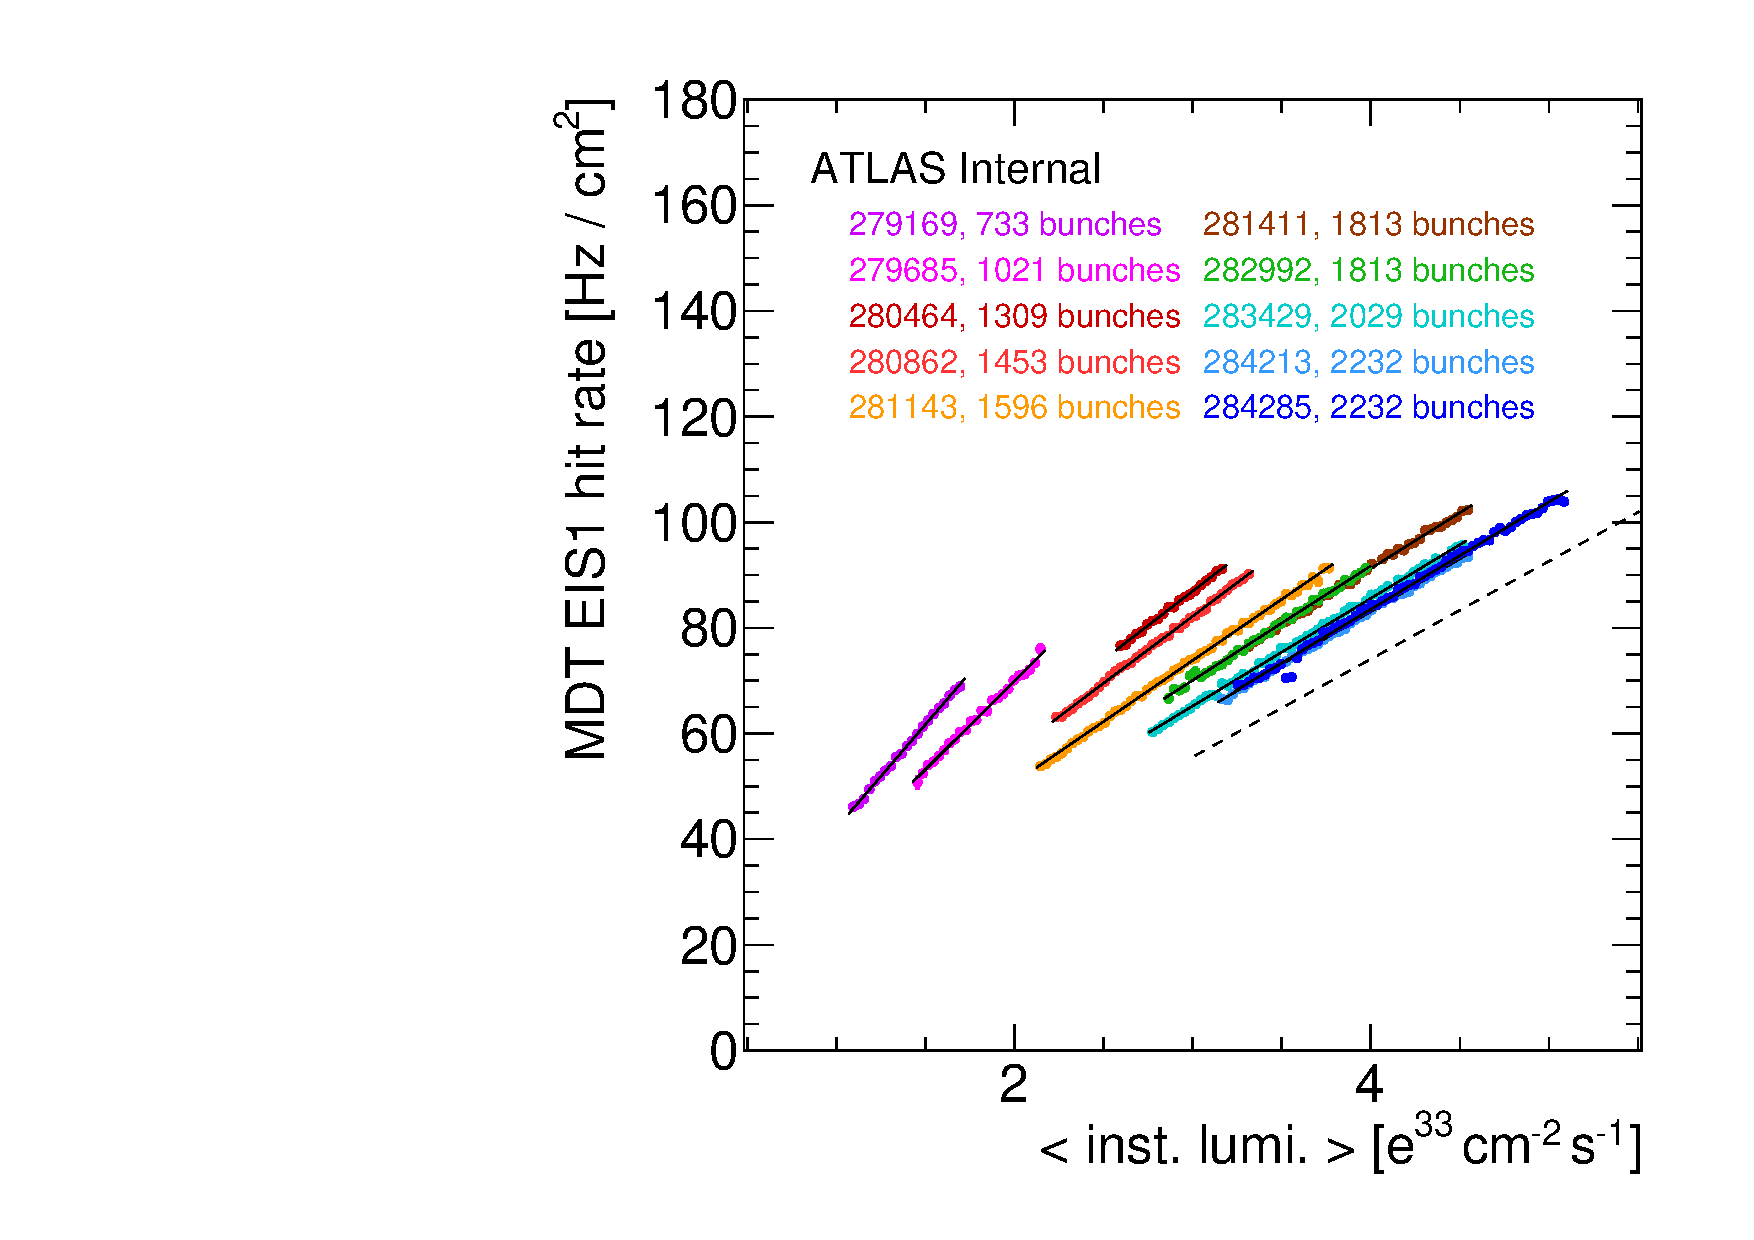
\includegraphics[width=0.45\textwidth]{./figures/rate_raw_vs_lumi_vs_evts_mdt_EIS1_overlay.pdf}
    \caption{Total hit rate in the hottest MDT chambers as a function of instantaneous luminosity, for multiple runs.}
    \label{fig:hitrates-vs-lumi-mdt-raw}
  \end{center}
\end{figure}

\begin{figure}
  \begin{center}
    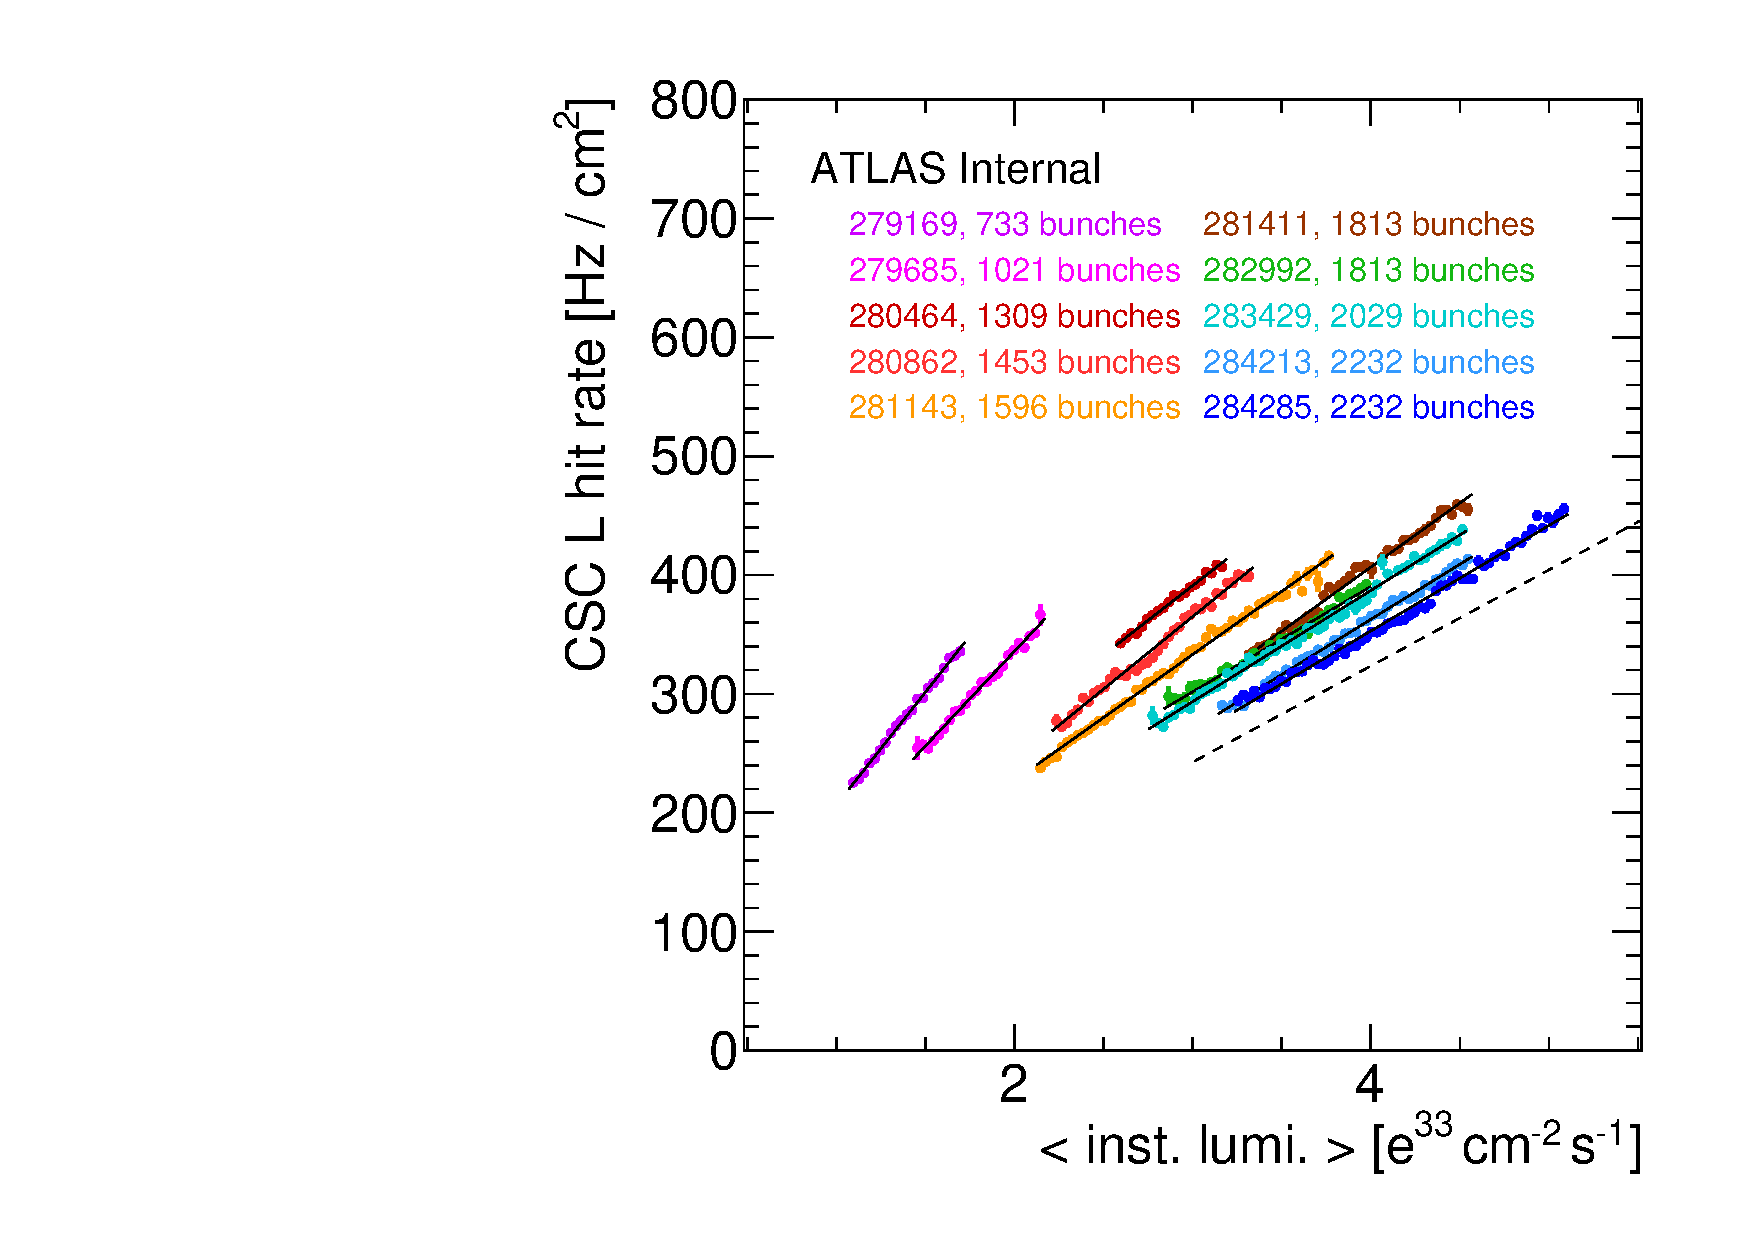
\includegraphics[width=0.45\textwidth]{./figures/rate_raw_vs_lumi_vs_evts_csc_CSL1_overlay.pdf}
    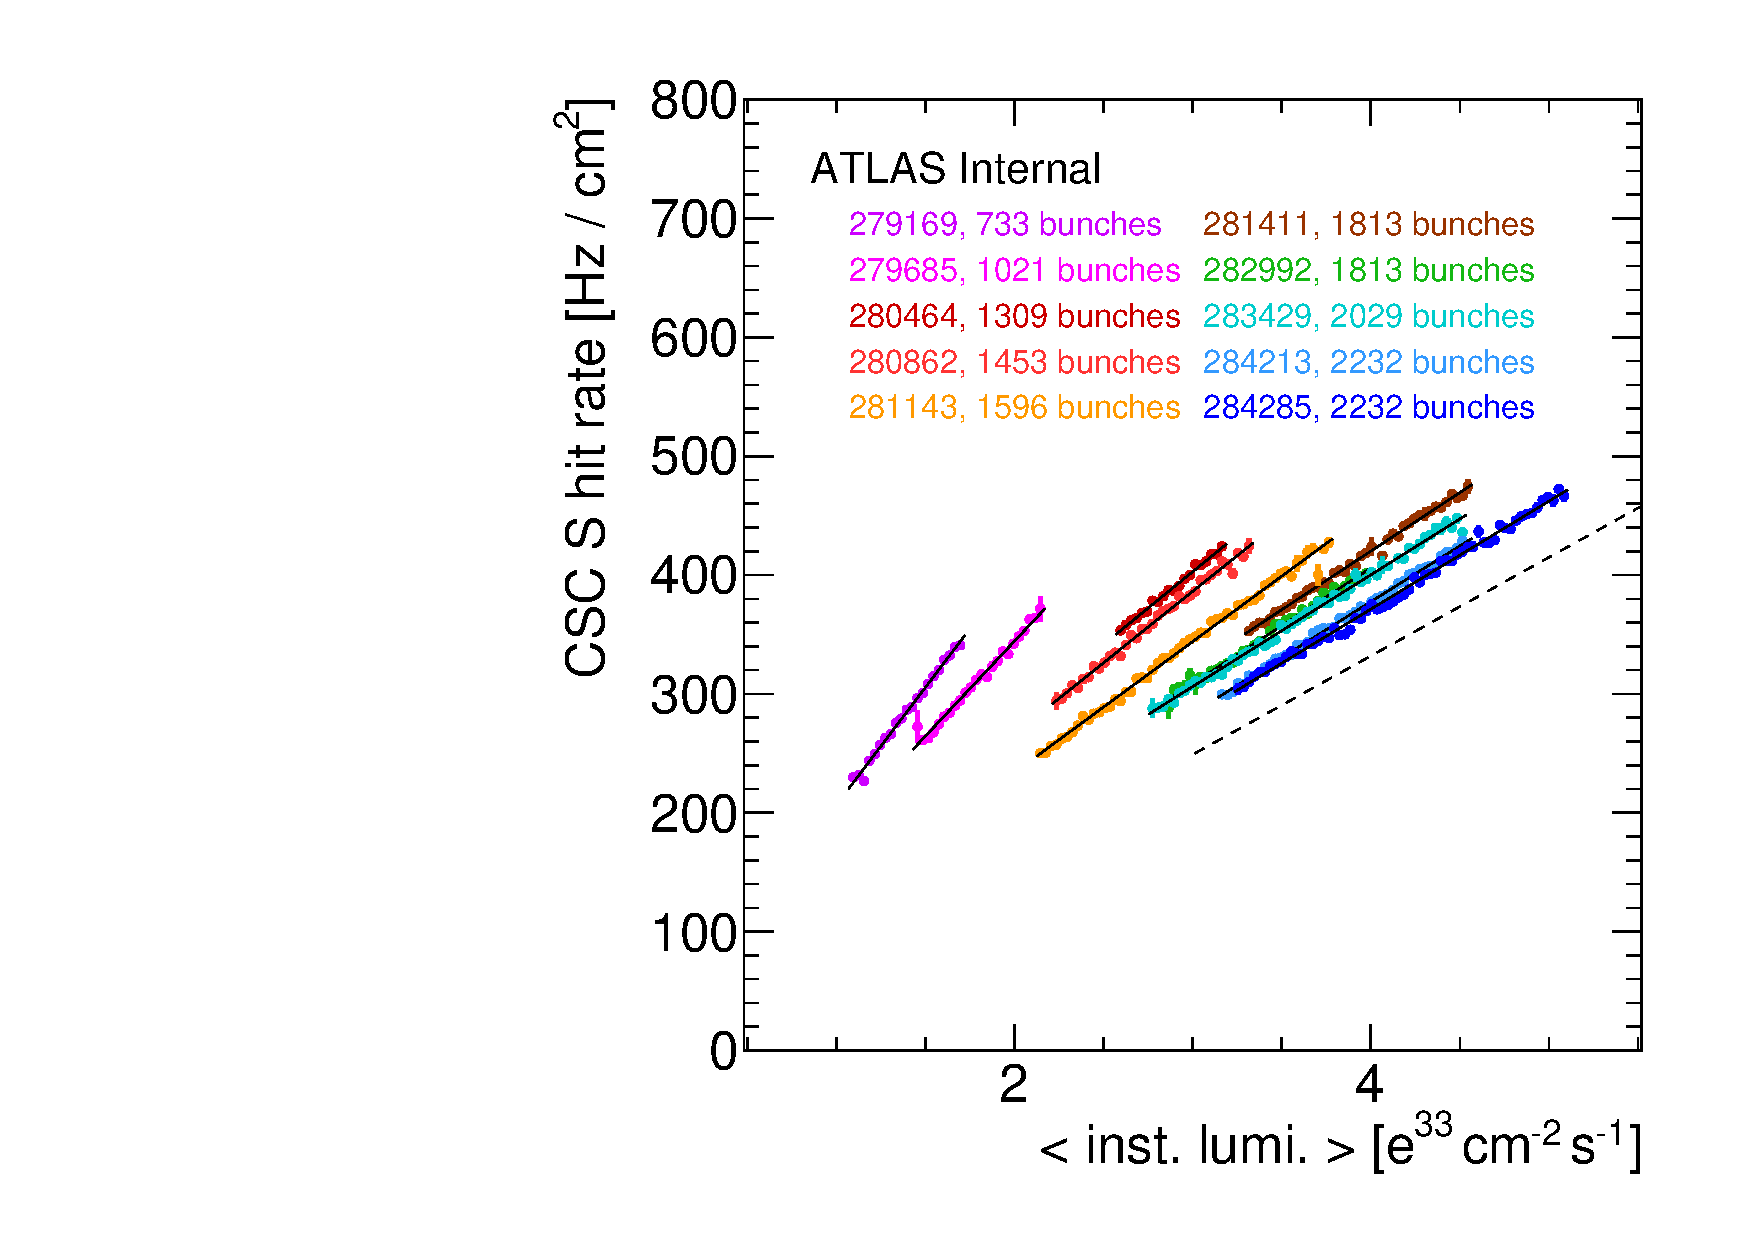
\includegraphics[width=0.45\textwidth]{./figures/rate_raw_vs_lumi_vs_evts_csc_CSS1_overlay.pdf}
    \caption{Total hit rate in the hottest CSC chambers as a function of instantaneous luminosity, for multiple runs.}
    \label{fig:hitrates-vs-lumi-csc-raw}
  \end{center}
\end{figure}

\begin{figure}
  \begin{center}
    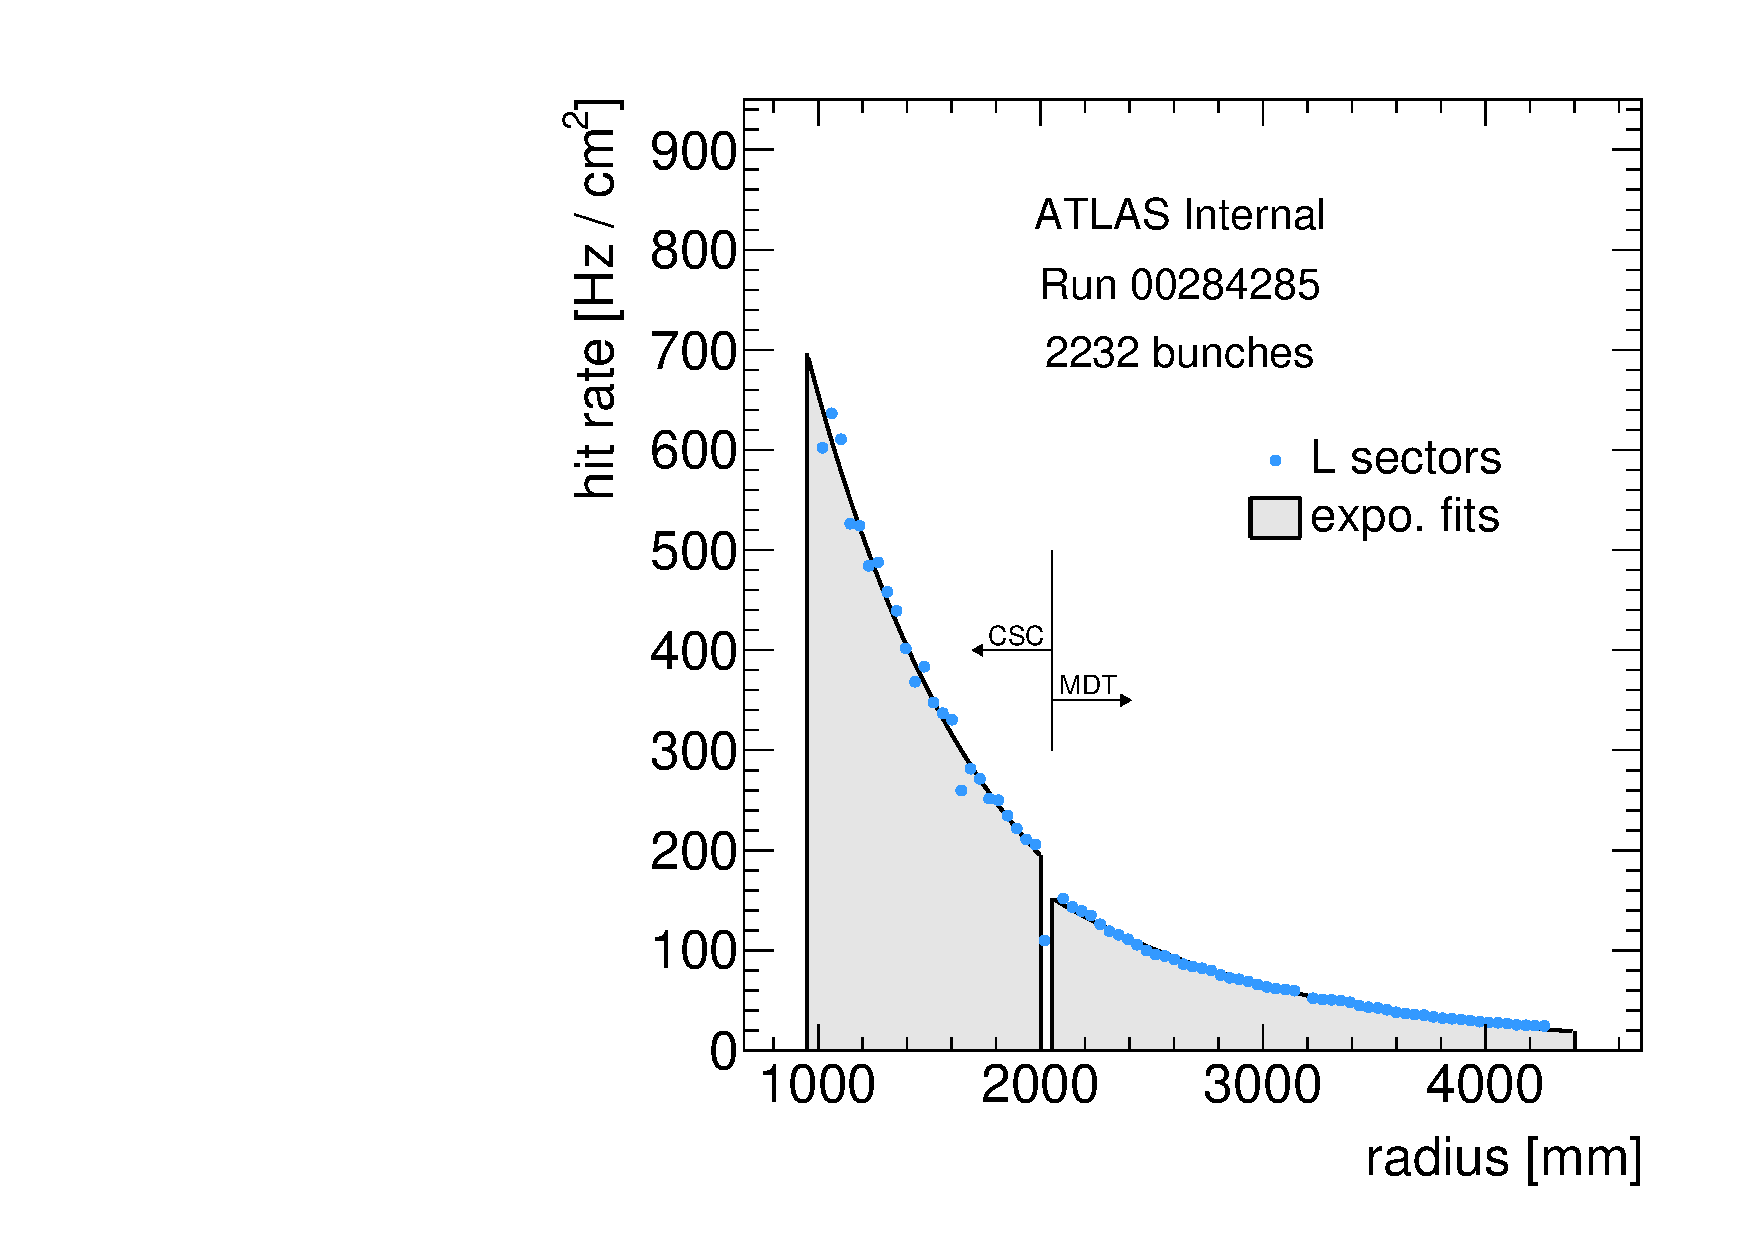
\includegraphics[width=0.45\textwidth]{./figures/rate_raw_vs_r_L_00284285.pdf}
    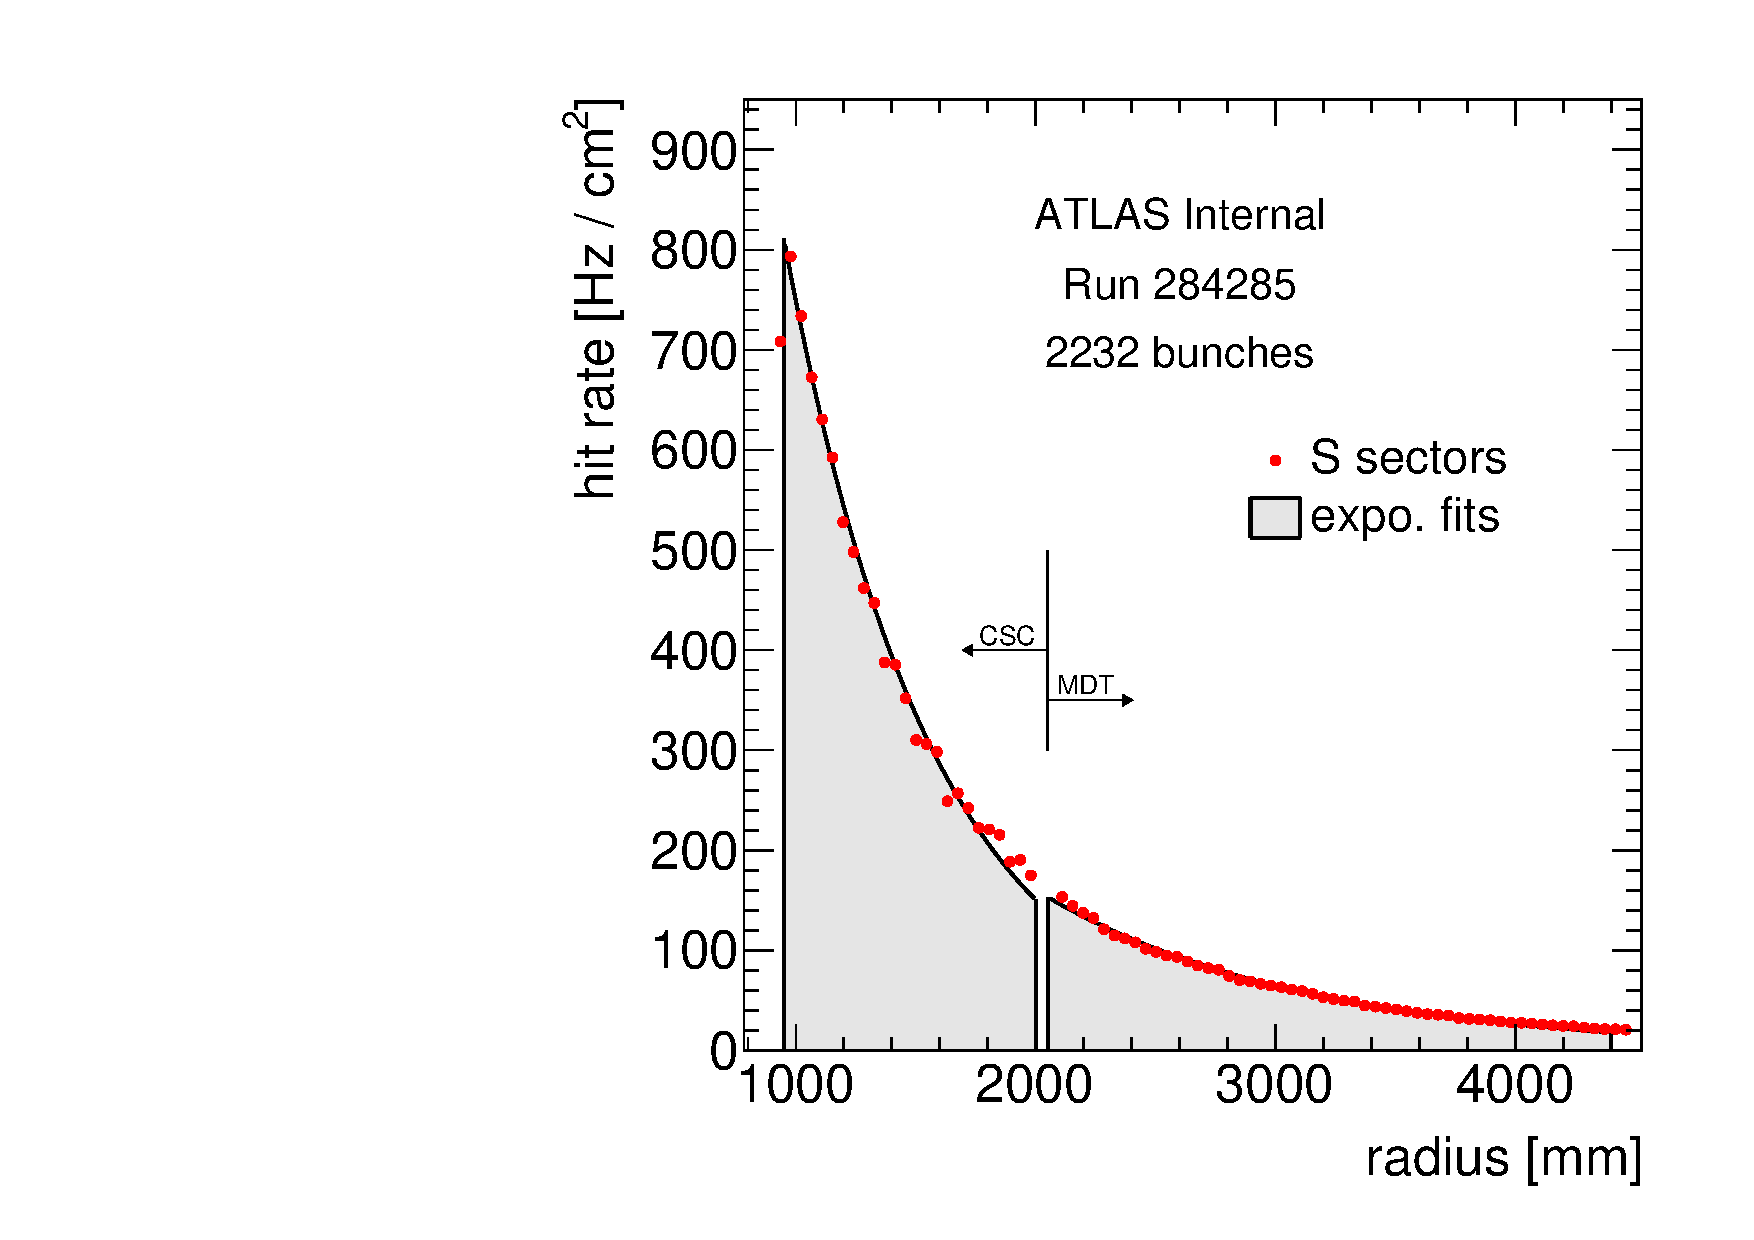
\includegraphics[width=0.45\textwidth]{./figures/rate_raw_vs_r_S_00284285.pdf}
    \caption{Total hit rate as a function of the transverse distance from the beam pipe in the small wheel, for large (left) and small (right) sectors, in Run 284285.}
    \label{fig:hitrates-vs-r}
  \end{center}
\end{figure}

